\documentclass[letterpaper,10pt]{article}

\usepackage{titling}
\usepackage{listings}
\usepackage{url}
\usepackage{setspace}
\usepackage{subfig}
\usepackage{sectsty}
\usepackage{pdfpages}
\usepackage{colortbl}
\usepackage{multirow}
\usepackage{relsize}
\usepackage{amsmath}
\usepackage{fancyvrb}
\usepackage{amsmath,amssymb,amsthm,graphicx,xspace}
\usepackage[titlenotnumbered,noend,noline]{algorithm2e}
\usepackage[compact]{titlesec}
\usepackage[default]{droidserif}
\usepackage[T1]{fontenc}
\usepackage{tikz}
\usetikzlibrary{arrows,automata,shapes,trees,matrix,chains,scopes,positioning,calc}
\tikzstyle{block} = [rectangle, draw, fill=blue!20, 
    text width=2.5em, text centered, rounded corners, minimum height=2em]
\tikzstyle{bw} = [rectangle, draw, fill=blue!20, 
    text width=4em, text centered, rounded corners, minimum height=2em]

\definecolor{namerow}{cmyk}{.40,.40,.40,.40}
\definecolor{namecol}{cmyk}{.40,.40,.40,.40}

\let\LaTeXtitle\title
\renewcommand{\title}[1]{\LaTeXtitle{\textsf{#1}}}


\newcommand{\handout}[5]{
  \noindent
  \begin{center}
  \framebox{
    \vbox{
      \hbox to 5.78in { {\bf ECE155: Engineering Design with Embedded Systems } \hfill #2 }
      \vspace{4mm}
      \hbox to 5.78in { {\Large \hfill #4  \hfill} }
      \vspace{2mm}
      \hbox to 5.78in { {\em #3 \hfill} }
    }
  }
  \end{center}
  \vspace*{4mm}
}

\newcommand{\lecture}[3]{\handout{#1}{#2}{#3}{Lecture #1}}
\newcommand{\tuple}[1]{\ensuremath{\left\langle #1 \right\rangle}\xspace}

\addtolength{\oddsidemargin}{-1.000in}
\addtolength{\evensidemargin}{-0.500in}
\addtolength{\textwidth}{2.0in}
\addtolength{\topmargin}{-1.000in}
\addtolength{\textheight}{1.75in}
\addtolength{\parskip}{\baselineskip}
\setlength{\parindent}{0in}
\renewcommand{\baselinestretch}{1.5}
\newcommand{\term}{Spring 2014}

\singlespace


\begin{document}

\lecture{ 21 --- Planning}{\term}{Patrick Lam}


\section*{Objectives}
After this lecture, you will be able to:
\begin{itemize}
\item distinguish between planning, scheduling and estimation;
\item identify the parts of a vision and scope document and a project plan;
\item participate in estimation processes and understand their components.
\end{itemize}

\section*{Planning and Estimation}
Planning is notoriously difficult to get right for software projects,
because estimates are always wrong.  We are going to look at
techniques which may help you better estimate, and hence plan,
your software projects.

\paragraph{Estimation.} An \emph{estimate} is an informed
guess, based on facts, about the amount of resources (primarily
effort/time) that a task will require to complete.

\paragraph{Planning.} When given a project to accomplish, 
the first thing to figure out is \emph{how} to do that project. We'll
call this \emph{planning}---dividing the project into a set of small,
related tasks. An important part of planning is identifying the
dependencies between the tasks, so that we can properly order them and
avoid unnecessary dependency-related delays.

{\sf What's an example of a plan?}
\vspace{5em}

\paragraph{Scheduling.} This is a more mechanical process. There can
be many valid ways to carry out a plan. When \emph{scheduling}, we propose
a particular order in which to carry out the plan. The inputs of scheduling
are a set of tasks, their dependencies, and estimates of the amount of
effort required. The output is a set of start and end times for each
subtask.

\paragraph{Recap.} Planning: figuring out \emph{how} to do a task, in terms of
breaking it down into subtasks. Scheduling: figuring out \emph{when}
to do the subtasks.

\section*{Planning}
A first, pre-planning, step in preparing for a project is to figure
out what the project entails. We will talk about the vision and scope document,
and then the different parts of the project plan.

\paragraph{Vision and Scope Document.} 
Writing this document helps you make sure that all of the
stakeholders, or people who need to care about the project, are on
board with the proposed project. You can think of this as preliminary
requirements gathering.The goal is to communicate with the stakeholders and, at a high
level, get them to sign off on what the project will and won't
include.

A \emph{vision and scope document} summarizes the design problem, the
stakeholders, the users, the risks, the assumptions, and the desired
features of a solution. In particular, it:
\begin{itemize}
\item identifies the features that will be included;
\item discusses features that stakeholders might expect but aren't slated
for inclusion (in this iteration);
\item summarizes agreed-upon expectations about the project's scope.
\end{itemize}
Project proposals are similar to vision and scope documents.

Here is a potential outline and example points for a vision and scope
document:
\begin{itemize}
\item Problem Statement: The project will develop a research prototype for a
better mousetrap.
\item Project Background: [Some paragraphs briefly discussing the
  current state of the art in mousetrap design.]
\item Stakeholders: The ACME Corporation eventually aims to sell these
  mousetraps to end users.
\item Users: End users will deploy the mousetraps in mouse-infested
  locations.
\item Risks: Mousetrap technology is a mature area, and many inventors
  have already attempted to develop better mousetraps, so this project
  may not successfully invent a better mousetrap.
\item Assumptions: The engineers have access to modern CAD software, a
  machine shop, and commonplace electronic components, for building
  their better mousetrap. The engineers' toy mice accurately represent
  the behaviour of actual real-world mice.
\item Vision of the Solution: The better mousetrap will use modern
  embedded systems technology, including sensors and actuators, to 
  effectively detect and trap mice without harming them.
\item List of features: The mousetrap will be able to detect and capture
  mice. Users will be able to calibrate the mousetrap for their intended
  deployment area. The mousetrap will include a provision for including 
  mousebait.
\item Scope of phased release: The first version of the mousetrap will
  detect mice, but will not capture the mice. The second version will
  detect and capture mice.
\item Features not to be developed: It remains the responsibility of the
  end-user to relocate the mice that this mousetrap catches.
\end{itemize}

\paragraph{Project Plan.} OK, so you have your vision and scope document.
Now you can start figuring out what you're going to need to do to
carry out the vision in the vision and scope document. 

The \emph{project plan} enumerates the work to be done on the project,
as well as who is to do the work. It has the following components:

\begin{itemize}
\item Statement of Work: describes all work projects to be produced,
  and identifies the people who will do work.
\item Resource List: contains a list of all resources needed for
the project and summarizes resource availability.
\item Work Breakdown Structure (WBS): describes all project activities.
\item Project Schedule: estimates start and end times for project activities.
\item Risk Plan: describes anticipated risks, likelihood of their occurrence,
and how to mitigate them.
\end{itemize}

\subsection*{Statement of Work}
A \emph{statement of work} (SOW) describes all work products to be
produced and identifies who will do the work.

This statement includes:
\begin{itemize}
\item a list of all project features that will be developed;
\item a description of each deliverable that will be developed (at
  this stage, one paragraph per deliverable); and
\item the estimated effort required for each deliverable, if known.
\end{itemize}

\subsection*{Resource List}

A \emph{resource list} enumerates all resources required for the
project and summarizes the availability of the resources.

A \emph{resource} is a person, a hardware component, a software
licence, a room, or anything else that is necessary for the project
but limited in availability.

The resource list is often maintained in a spreadsheet or a database,
and contains records consisting of:
\begin{itemize}
\item resource name;
\item a brief (one-line) description of the resource; 
\item a summary of resource availability (start dates, end dates, etc.); and
\item the cost of the resource (if applicable).
\end{itemize}

\subsection*{Work Breakdown Structure (WBS)}
A \emph{work breakdown structure} (WBS) describes all project
activities.  That is, it comprehensively lists all project activities
required to complete the project, including intermediate deliverables.
The WBS needs to evolve as the project becomes better-defined and more
details about required project activities become known.

Revision control (like Subversion) is also appropriate for
non-software products, like WBSes, which are expected to evolve over
time. Future project planning may benefit from studying the revision
history of similar projects which happened in the past.

The \emph{Software Project Management} textbook describes the
``Wideband Delphi Process'' for estimating the time required for each
activity in a WBS.

\subsection*{Project Schedule}
A \emph{project schedule} estimates start and end times of all project
activities. These estimates should be developed using a repeatable,
defensible process.

One way of getting estimates is by running meetings where participants
defend their estimates.
\begin{enumerate}
\item Each participant writes down an initial estimate, along with assumptions,
for each project activity.
\item A moderator collects all estimates and summarizes them.
\item The participants discuss the estimates.
\item Repeat as needed.
\end{enumerate}

Documenting assumptions helps refine estimates and reduce variance in
estimates. Although the participants may not reach consensus, the resulting
estimates should at least not differ too radically.

\subsection*{Risk Plan}
Recall that a risk is a potential threat to the successful completion
of your project. A \emph{risk plan} therefore describes anticipated
risks, the likelihood of their occurrence, and how they might be
handled. Good risk plans are comprehensive and include potential ways
to mitigate significant risks.

The risk plan is usually developed in a risk assessment and planning session:
\begin{itemize}
\item Team members brainstorm to create a list of potential risks that threaten the project.
\item For each risk, team members estimate the likelihood of the risk and its potential impact.
\item Taking likelihood and impact into account, team members develop a plan for mitigating each risk.
\end{itemize}

\paragraph{Risk Plan Example.} See page 29 of \emph{Applied Software Project
Management} for a sample risk plan.

\section*{Estimates}
Project plans include project schedules, which estimate how long
everything takes. Estimates are notorious for being wrong (and not in
the good way).  However, this may help you come up with accurate time
estimates:

\begin{itemize}
\item An accurate work breakdown structure for the project.
\item An effort estimate for each task listed in the work breakdown structure.
\item A list of the assumptions made during the establishment of the effort estimates.
\item Consensus among the members of the project team that effort estimates are reasonable.
\end{itemize}

\paragraph{On Assumptions.} Do assumptions make estimates less accurate?
Not necessarily! Unstated assumptions, however, are troublesome.

If an assumption is well-documented and properly communicated, it can
improve the quality of an estimate:
\begin{itemize}
\item it may reveal an non-obvious problem or detail;
\item it may reveal a simplification that some, but not all, members of the estimation team were relying on; and,
\item finding out that an assumption is untrue is a good time to revisit an estimate.
\end{itemize}

Agreeing on a common set of assumptions allows the estimation team to 
move beyond the assumptions and come up with good estimates.

%% Assumptions also allow the estimation team to skip over irrelevant
%% details and focus on the important decisions that will affect
%% development.

\paragraph{Padding Estimates.}  (``Scotty Time\footnote{\url{http://tvtropes.org/pmwiki/pmwiki.php/Main/ScottyTime}}''). Padding an estimate seems like all win: underpromise and overdeliver, etc. This is, however, not necessarily a good idea. Let's talk about the benefits and costs of this approach.

% 14:55 at http://www.youtube.com/watch?v=LdShpVwQr9s

Benefits:
\begin{itemize}
\item You look like a hero by doing better than you said you would.
\item Working based on padded time estimates helps you alleviate time pressures.
\end{itemize}

Problems:
\begin{itemize}
\item You can only look like a hero a couple of times before you look like a zero and managers adapt to your padded estimates. (Managers aren't dumb.)
\item Managers don't trust engineers who habitually pad time estimates.
\item Clients or managers may decide to not proceed based on the too-expensive padded estimate.
\end{itemize}

\section*{Estimation Techniques}
We are going to talk about a number of estimation techniques, including the
Wideband Delphi Process, PROBE, COCOMO II, and The Planning Game.

\subsection*{Wideband Delphi Process}
 
This repeatable process consists of a set of straightforward steps:
\begin{itemize}
\item Choose an estimation team and moderator.
\item Hold a kickoff meeting to develop a work breakdown structure, a preliminary list of assumptions, and a unit of estimation.
\item Allow estimation team members to independently prepare estimates for each task and prepare a list of additional assumptions.
\item Hold an estimation session, where the moderator requests estimates from team members, and attempts to achieve consensus on estimates by having members explain their estimates.
\item Assemble the final list of tasks and estimates.
\item Review the results with the project manager and the estimation team.
\end{itemize}
Note that estimation sessions are key to the Wideband Delphi Process.

\paragraph{Starting an Estimation Session.}
First, team members share effort estimates for each task in the work
breakdown structure. The moderator records these estimates and plots
them on a graph or records them in a table. One might expect the
range of these estimates to be large, because team members may make
different assumptions. See below (graphics from \cite{aswpm}):

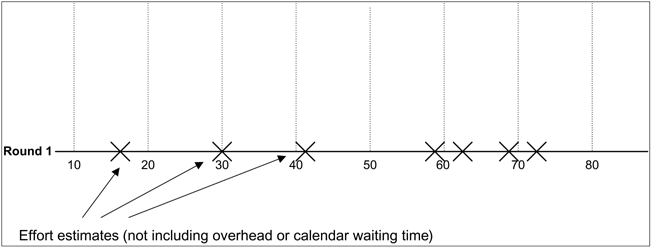
\includegraphics[width=\textwidth]{images/effort-estimates.png}

\paragraph{Achieving consensus.} The point of working in a team is
to come up with a consensus which is, ideally, better than the results
that individual members would have come up with. The Wideband Delphi 
Process uses a number of rounds of discussion in the estimation session.
In each round, team members discuss assumptions, clarify
project details, and revise estimates. Here's an example of convergence
in estimates:

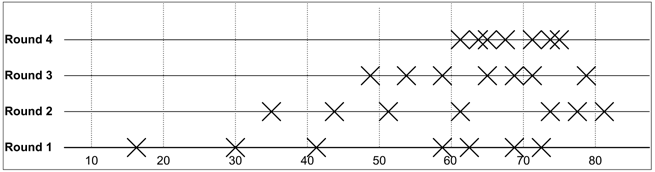
\includegraphics[width=\textwidth]{images/converging-effort-estimates.png}

\section*{Other Estimation Techniques}
There are a number of estimation techniques besides Wideband Delphi.
Here are some well-known estimation techniques for software.

\paragraph{PROBE.} It's sensible to believe that if you're doing something
similar to something that you've done in the past, it should take about
the same amount of time. So, the idea here is to obsessively track
how long it took to do things in the past, and then use linear
regression to estimate how long it'll take in the future. 

{\sf What are some potential problems with this technique?}\\[3em]

% killer overhead, doesn't necessarily generalize, 
% doesn't work well for newbies.

\paragraph{COCOMO II.} The idea here is to feed in a number of guesses
about your project's scope, apply a formula full of fudge factors
(developed based on empirical data), and get an estimate of size and
effort. Examples of guesses include memory constraints, analyst
capability, and product complexity.  COCOMO stands for
\emph{COnstructive COst MOdel}.

\subsection*{The Planning Game} 
This isn't one of those fun games like Mass Effect. Instead, it's an
estimation technique developed by Kent Beck (inventor of extreme
programming) while working at Chrysler in the 1990's.

The \emph{Planning Game} is a planning process that 1) identifies
the scope of the project as well as 2) the tasks required to complete
the project. It also 3) estimates the effort required for these tasks.
This game consists of two phases: release planning and iteration planning.
Release planning plans the scope of the project, while iteration
planning plans the activities and tasks of the developers. The Planning
game requires a team consisting of customers and developers.

\paragraph{Release Planning.} 
Each week, the team meets to plan the immediate future of the project.
The team writes user stories describing project requirements on index cards,
and assigns effort estimates for the stories (e.g., 1, 2, or 3 weeks).
The team prioritizes the requirements.

\paragraph{Iteration Planning.} 
The team divides requirements into sets of tasks to be completed.
It then assigns these tasks to developers, and estimates effort
for these tasks. Developers complete these tasks and match them
back up with the user stories.


\bibliographystyle{alpha}
\bibliography{155}


\end{document}
